\documentclass[11pt]{article}
\usepackage{icmlko}
\begin{document}

\title{수집이 끝나기 전에 위약을 재면 안 된다 --- 애니 아카이브 1,312편}
\author{월드모델 실험실}
\date{노트 394 · 2026년 8월 1일}
\maketitle

\begin{abstract}
노트 387이 웹툰 아카이브로 판을 올렸고, 노트 388이 그 이득의 출처를 학습
라벨 범위로 좁혔다. 같은 자리가 애니에 더 크게 있었다 --- 라프텔 목록
9,472편 중 우리가 2,073편(덮음 \textbf{22\%})이고, 우리 표본은 오프셋 0
근처(최신)에 몰려 있다.

1,312편(전부 2025년 이전)을 받아 \textbf{학습에만} 더했다. 유보 606행은
두 팔이 같다.

\begin{center}
\textbf{판 짝 12뽑기 $+0.0073$ · 12/12 · 애니 $+0.0444$ · 12/12}, 조건 ②
열한 도메인 전부 통과 $\Rightarrow$ \textbf{채택}
\end{center}

\textbf{그런데 이번 노트의 값은 채택이 아니라 세 번 걸려 넘어진 자리다.}

\textbf{첫째, 위약 잔량이 수집 중에 크게 움직인다.} 노트 390의 사전 계산은
``기존 범위 밖 0\% $\Rightarrow$ 위약 잔량 0\% 근처''를 예측했는데, 같은
실험을 새 행 1,086 / 1,186 / 1,312 개로 재니 잔량이
\textbf{35\% $\to$ 19\% $\to$ 6\%} 다. \textbf{첫 수치로 노트 390을
반증하는 노트를 쓸 뻔했다.} 위약 잔량은 관문 \emph{둘}의 차이라 잡음이
두 배로 실린다 --- 수집이 끝난 뒤에 재야 한다.

\textbf{둘째, 관문을 돌린 표본과 채택한 표본이 달랐다.} 수집기가 배경에서
계속 돌아, 1,186편으로 관문을 돌리고 1,312편을 넣었다. \textbf{단일 적합
판이 내려간 것으로 잡았다} --- 되돌리고, 수집기를 멈춰 표본을 고정하고,
같은 표본으로 다시 쟀다.

\textbf{셋째, 내 위험 점검 코드가 마지막 팔 뒤에 돌았다.} 이번 관문에는
위약2 팔(옛 라벨을 일부러 맞바꾸는 팔)이 있어서 ``옛 행 라벨 1,309개
바뀜''으로 보였다. 백업 대 채택본으로 다시 세니 \textbf{0행}이다.

두 위약이 둘 다 필요했다 --- 위약1 잔량 6\%(행 수준 정보), 위약2
$-1290$\%(무리 수준도 정보). \texttt{venue\_prominence} 가 백분위라 옛 행의
42\%가 움직이는데, 양쪽에서 막아도 이득의 86\%가 남으므로 원인이 아니다.
\end{abstract}

\section{쟀다}

\texttt{ingest/anime\_more.py} 로 라프텔 목록 전체(9,472)를 훑어 우리가 없는
것을 모으고, \textbf{씨앗으로 섞어}(노트 383) 상세를 받았다. 1,466편 중
2025년 이전 1,312편이 학습 후보다.

\textbf{노트 390의 요청 없는 사전 계산부터 했다.} 새 행의 라벨이 기존 학습
범위(한줄평 1\,--\,2,951) \emph{밖}에 있는 비율이 \textbf{0\%} 다 ---
범위가 통째로 겹친다. 그러면 위약1(새끼리 섞기)이 옳은 검사이고 잔량이
0\% 근처로 나와야 한다.

\begin{center}
\begin{tabular}{lrrr}
\hline
팔 & 판 차 & 부호 & 애니 차 \\
\hline
B 아카이브 더함 & $+0.0073$ & \textbf{12/12} & $+0.0444$ (12/12) \\
C 위약1 (새끼리 섞기) & $+0.0016$ & 7/12 & $+0.0028$ (6/12) \\
D 위약2 (옛 것과 맞바꿈) & $-0.1062$ & 0/12 & $-0.5730$ (0/12) \\
\hline
\end{tabular}
\end{center}

\textbf{위약1 잔량 6\%} --- 사전 계산대로다. 그리고 위약2 를 붙여 보니
$-1290$\% 로, 무리 수준 연합도 실재하는 정보다(노트 392의 절차).

\textbf{조건 ②} 열한 도메인 중 $|t|>2.77$ 로 나빠진 것이 없다(제일 나쁜
도서 $-0.0259$, SD 0.0382, $|t|{=}0.68$). 부호가 12/12 라 노트 378 조항
①로 \textbf{판이 직접 채택}한다.

\begin{figure}[t]
\centering
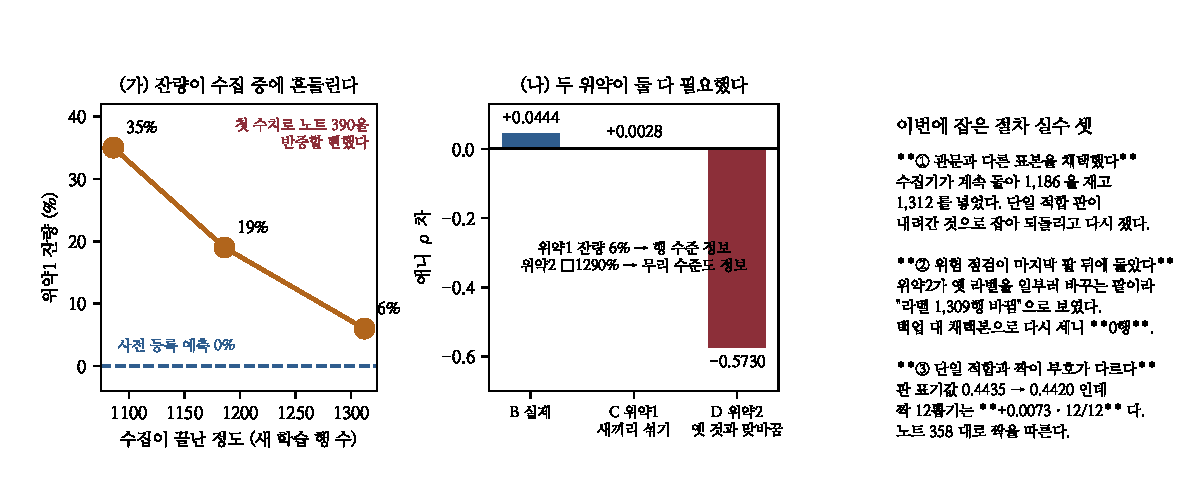
\includegraphics[width=\linewidth]{figs/fig394.pdf}
\caption{\textbf{(가)} 같은 실험의 위약1 잔량이 수집이 진행되면서
35\% $\to$ 19\% $\to$ 6\% 로 내려간다. \textbf{(나)} 두 위약. 위약1은
6\%만 남기고 위약2는 뒤집는다. \textbf{(다)} 이번에 잡은 절차 실수 셋.}
\label{fig:main}
\end{figure}

\section{잔량이 움직인다}

이 노트를 처음 쓸 때는 제목이 ``노트 390의 사전 계산이 반증됐다''였다.
새 행 1,086개로 잰 위약1 잔량이 \textbf{35\%} 였기 때문이다 --- 밖 비율
0\%가 예측한 값의 정반대다. 분포를 보니 그럴듯한 설명까지 있었다: 범위는
겹치는데 새 행의 라벨 중앙이 148 대 14 로 \textbf{10.6배} 아래이고(MWU
$p{=}3{\times}10^{-176}$) 시작 연도 중앙은 2021 대 2020 으로 같으니,
``범위가 아니라 분포''라고 쓰면 됐다.

\textbf{그런데 수집이 더 진행된 뒤 다시 재니 19\%, 다 끝내고 재니 6\%
였다.} 35\%는 잡음이었다.

\textbf{왜 이렇게 흔들리나.} 위약 잔량은 \emph{두 관문의 비}다 ---
$(\text{위약} - A) \div (\text{실제} - A)$. 분자와 분모가 각각 짝지은
12뽑기의 평균이라 각자 잡음을 갖는데, 분모가 작으면(여기서 애니 차가
$+0.04$ 수준) 비가 크게 튄다. \textbf{잔량은 판 차보다 훨씬 불안정한
수다.}

\textbf{규약에 적는다: 위약 잔량은 수집이 끝난 뒤에 잰다.} 진행 중에 잰
값으로 규칙을 세우거나 반증하지 않는다. 노트 390이 자기 대응을
``법칙이 아니라 검사해야 할 관측''이라 못 박아 둔 것이 이번에 값을 했다
--- 그 문장이 없었으면 35\%를 근거로 대응을 버렸을 것이다.

\section{나머지 두 실수}

\textbf{표본이 움직이는 채로 채택했다.} 수집기가 배경에서 계속 돌고
있어서, 1,186편으로 관문을 돌린 뒤 채택할 때는 1,312편이 되어 있었다.
잡은 것은 \textbf{단일 적합 판이 0.4435에서 0.4420으로 내려간 것}이다 ---
짝 12뽑기가 $+0.0073$ 인데 단일 적합이 내려가면 둘 중 하나가 다른 자료를
보고 있다는 뜻이다. 되돌리고, 수집기를 멈추고, 고정된 1,312편으로 다시
쟀다. \textbf{규약: 관문을 돌리기 전에 수집기를 멈춰 표본을 고정한다.}

\textbf{위험 점검이 엉뚱한 것을 쟀다.} 점검 코드가 팔을 다 만든 \emph{뒤에}
축 파일을 읽는데, 이번 관문의 마지막 팔이 위약2 --- 옛 행의 라벨을 일부러
맞바꾸는 팔 --- 이라 ``옛 행 라벨 1,309개 바뀜''이 찍혔다. 웹툰 · 만화
관문에는 위약2 팔이 없어서 안 걸렸던 버그다. 백업 대 채택본으로 직접
세니 \textbf{라벨 0행 · 축 넷 100\% 그대로}다.

\textbf{남은 것 하나는 진짜다:} \texttt{venue\_prominence} 는 표본 안
백분위라 행을 63\% 더하니 옛 행의 42\%가 움직인다($|$차$|$ 평균 0.073 ·
최대 0.76). 노트 387이 웹툰에서 한 대조를 그대로 했다 --- 양쪽에서 막고
재면 판 $+0.0063$ · 11/12 로 \textbf{이득의 86\%가 남는다.} 원인이 아니다.

\section{단일 적합과 짝이 부호가 다르다}

\begin{center}
\begin{tabular}{lrr}
\hline
 & 단일 적합 판 & 짝 12뽑기 \\
\hline
채택 전 & 0.4435 & --- \\
채택 후 & \textbf{0.4420} & $\mathbf{+0.0073}$ (12/12) \\
\hline
\end{tabular}
\end{center}

\textbf{표기값은 내려가는데 짝은 12/12 로 오른다.} 노트 358이 ``한 번
적합은 도메인 부호가 열에 넷 틀린다''를 쟀으니 짝을 따른다. 다만
\textbf{대장에 둘 다 적는다} --- 이번 사이클에서 채택한 변경 중 두 수의
부호가 갈린 것은 이번이 처음이다.

\section{남은 것}

\begin{center}
\begin{tabular}{lll}
\hline
항목 & 왜 값이 큰가 & 어떻게 \\
\hline
애니 나머지 & 덮음 22\% $\to$ 36\% 까지만 왔다 & 수집 재개(목록 9,472) \\
잔량의 잡음 폭 & 얼마나 흔들리는지 안 쟀다 & 같은 자료로 씨앗만 바꿔 열 번 \\
표기값 대 짝 & 부호가 갈리는 조건 & 지난 채택들에 소급 \\
웹툰 835 안/밖 & 아직 안 갈랐다 & 위약1 · 위약2 각각 \\
\hline
\end{tabular}
\end{center}

\end{document}
